\subsection{Collie River Basin 3 (model ID: 11)}
The Collie River Basin 3 model (fig.~\ref{fig:11_schematic}) is part of a top-down modelling exercise and is originally applied at the daily scale \citep{Jothityangkoon2001}. It has 2 stores and 6 parameters ($S_{max}$, $S_{fc}$, $a$, $M$, $b$, $\lambda$). The model aims to represent:

\begin{itemizecompact}
\item Separate bare soil and vegetation evaporation;
\item Saturation excess surface runoff;
\item Non-linear subsurface runoff;
\item Non-linear groundwater runoff.
\end{itemizecompact}

\subsubsection{File names}
\begin{tabular}{@{}ll}
Model: &m\_11\_collie3\_6p\_2s \\
Parameter ranges: &m\_11\_collie3\_6p\_2s\_parameter\_ ranges \\
\end{tabular}

% Equations
\subsubsection{Model equations}

% Model layout figure
{ 																	% This ensures it doesn't warp text further down
\begin{wrapfigure}{l}{5cm}
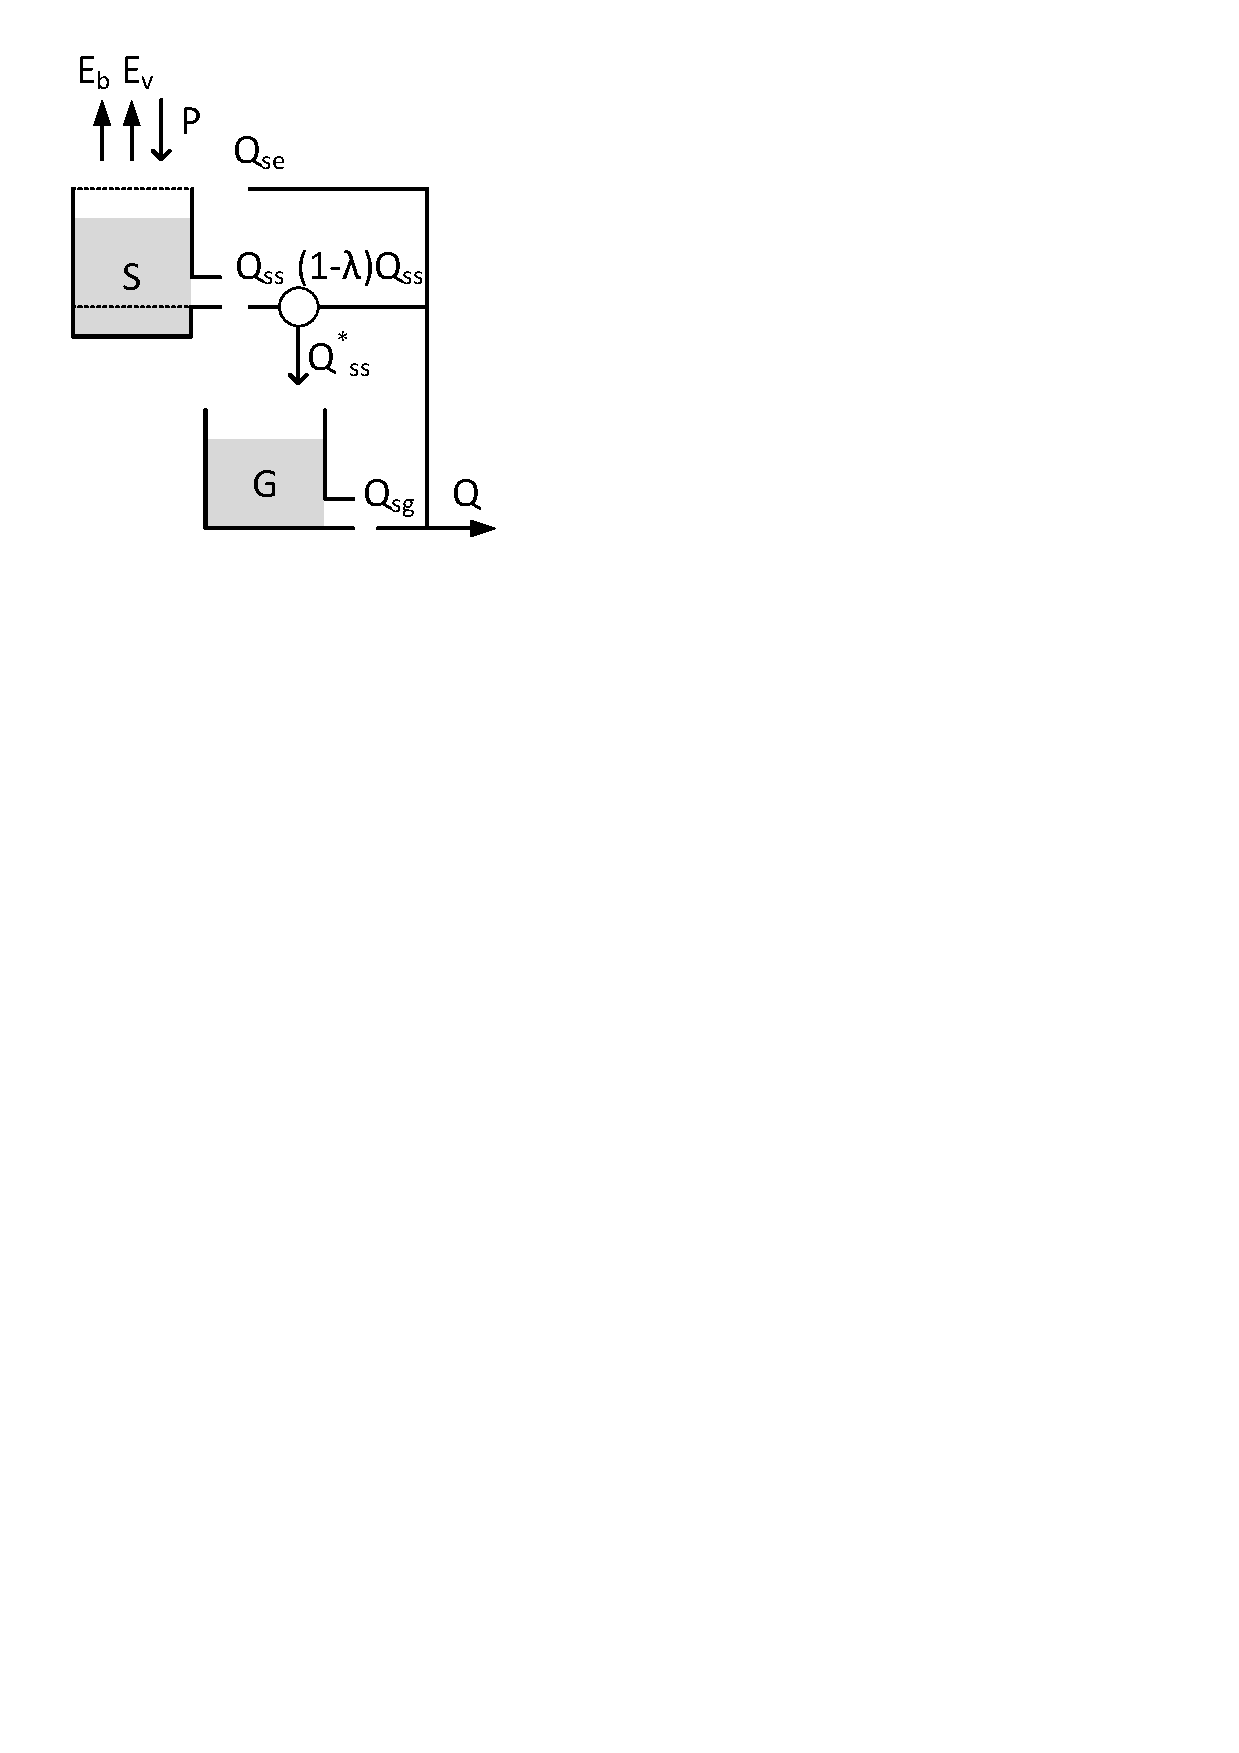
\includegraphics[trim=1cm 20cm 9cm 1cm,width=7cm,keepaspectratio]{./files/11_schematic.pdf}
\caption{Structure of the Collie River Basin 3 model} \label{fig:11_schematic}
\end{wrapfigure}

\begin{align}
	\frac{dS}{dt} &= P -E_b - E_v -Q_{se}-Q_{ss} \\
	Eb &= \frac{S}{S_{max}}(1-M)*Ep\\
	Ev &= 
		\begin{cases}
			M*E_p, & if~S>S_{fc}\\
			\frac{S}{S_{fc}}*M*E_p, &otherwise\\
		\end{cases}\\
	Q_{se} &= 
		\begin{cases}
			P, & if~S>S_{max}\\
			0, & otherwise \\
		\end{cases}\\
	Q_{ss} &= 
		\begin{cases}
			\big(a*(S-S{fc})\big)^b, & if~S>S_{fc}\\
			0, & otherwise 
		\end{cases}
\end{align}
}
\vspace{1.5cm}

Where  $S$ [mm] is the current storage in the soil moisture and $P$ the precipitation input $[mm/d]$. Actual evaporation is split between bare soil evaporation $E_b$ $[mm/d]$ and transpiration through vegetation $E_v$ $[mm/d]$, controlled through the forest fraction $M$. The evaporation estimates are based on the current storage $S$, the potential evapotranspiration $E_p$ $[mm/d]$ and the maximum soil moisture storage $S_{max}$ [mm], and field capacity $S_{fc}$ [mm] respectively. $Q_{se}$ $[mm/d]$ is saturation excess overland flow.  $Q_{ss}$ $[mm/d]$ is non-linear subsurface flow regulated by runoff coefficients $a$ $[d^{-1}]$ and $b$ [-].

\begin{align}
	\frac{dG}{dt} &= Q_{ss}^* - Q{sg} \\
	Q_{ss}^* &= \lambda*Q_{ss} \\
	Q_{sg} &= (a*G)^b
\end{align}

Where $G$ [mm] is groundwater storage. $Q_{ss}^*$ $mm/d]$ is the fraction $\lambda$ of $Q_{ss}$ directed to groundwater. $Q_{sg}$ $[mm/d]$ is non-linear groundwater flow that relies on the same parameters as subsurface flow uses. Total runoff:

\begin{equation}
	Q = Q_{se} + (1-\lambda)*Q_{ss} + Q_{sg}
\end{equation}


\subsubsection{Parameter overview}
% Table generated by Excel2LaTeX from sheet 'Sheet1'
\begin{table}[htbp]
  \centering
    \begin{tabular}{lll}
    \toprule
    Parameter & Unit  & Description \\
    \midrule
    $S_{max}$ & $mm$  & Maximum soil moisture storage \\
    $S_{fc}$ & $mm$  & Field capacity \\
    $a$   & $d^{-1}$ & Runoff coefficient \\
    $M$   & $-$   & Forest fraction \\
    $b$   & $-$   & Runoff nonlinearity \\
    $\lambda$ & $-$   & Fraction subsurface flow to groundwater \\
    \bottomrule
    \end{tabular}%
  \label{tab:addlabel}%
\end{table}%
